\chapter{Używanie aplikacji}

W tym rozdziale opisano proces interakcji z różnymi funkcjami aplikacji i ich wpływ na końcowy wynik pracy na konkretnym przykładzie.

	\section{Przykład tworzenia workspace}
	
		Rozważmy sytuację, w której wybieramy film z YouTube do analizy. W niniejszym przykładzie rozważymy film, który jest przedstawiony na Rysunku \ref{fig:YouTubeVideoPreview}.
		
		\begin{figure}
			\centering
			\scalebox{1.0} {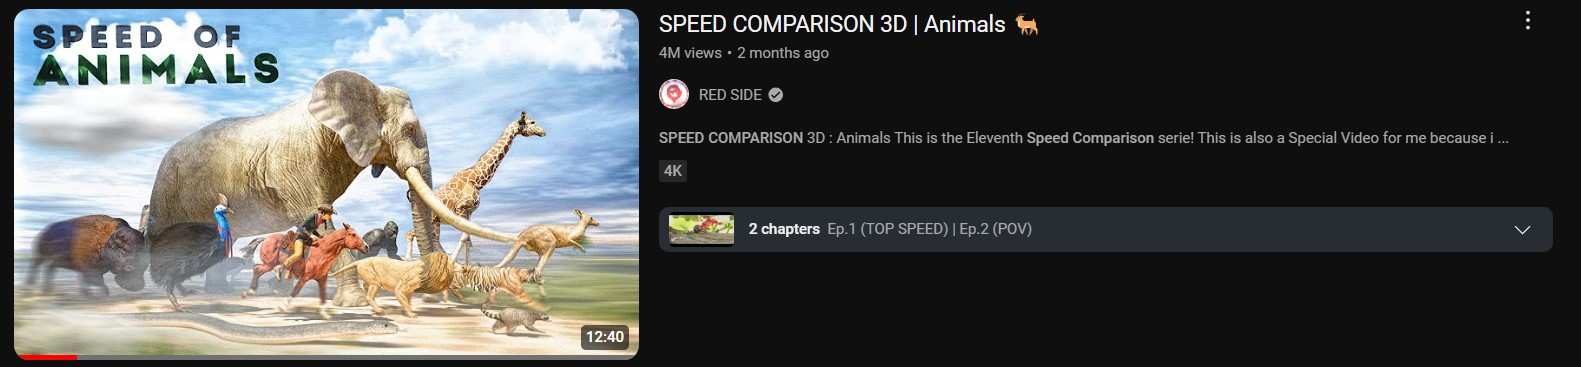
\includegraphics[width=0.5\textwidth]{./img/YouTubeVideoPreview.jpg}}
			\caption{Przykład filmu na YouTube.}
			\label{fig:YouTubeVideoPreview}
		\end{figure}
		
		\subsection{Pobieranie danych tekstowych}
		
		Pierwszym krokiem jest pobranie danych. Po uruchomieniu aplikacji należy otworzyć okno dialogowe YouTube Comments za pomocą paska menu \textbf{Comments} -- \textbf{YouTube}. Następnie należy wkleić link do filmu i kliknąć przycisk \textbf{Find Video}. Po tej operacji okno powinno wyglądać jak na Rysunku \ref{fig:YouTubeWindowThiContent}, gdzie wyświetlone są podstawowe informacje o filmie. Po potwierdzeniu, że to właściwy film, należy kliknąć przycisk \textbf{Download Comments}. Proces może chwilę potrwać w zależności od liczby komentarzy. Po zakończeniu pomyślnym zostanie wyświetlony komunikat \textbf{Comments downloaded successfully}, co oznacza, że komentarze zostały pobrane i zapisane w folderze \textbf{Comments} pod nazwą pliku \textbf{video\_id.txt}, w tym przykładzie jest to~~\textbf{90OC4TQ7uHc.txt}.
		
		\begin{figure}
			\centering
			\scalebox{1.0} {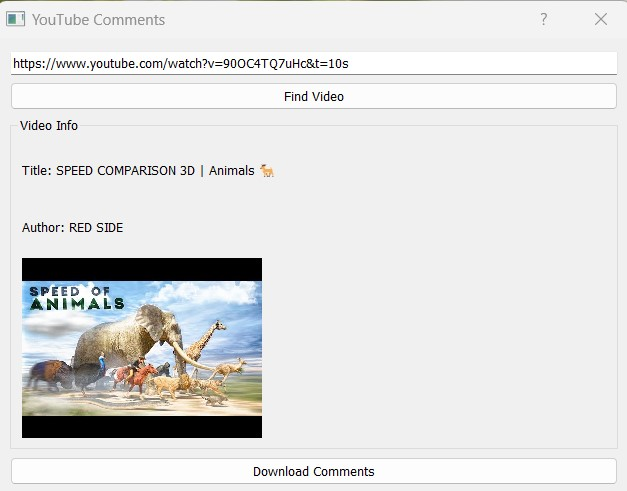
\includegraphics[width=0.5\textwidth]{./img/YouTubeWindowThiContent.jpg}}
			\caption{Przykład wypełnionego okna pobierania komentarzy.}
			\label{fig:YouTubeWindowThiContent}
		\end{figure}
		
		\subsection{Tworzenie Workspace}
		
		Aby utworzyć projekt(workspace) do pracy z pobranymi komentarzami, należy przejść do~~menu \textbf{File} -- \textbf{New Project}, gdzie można wprowadzić ścieżkę do pliku z danymi. Można również skorzystać z przycisku \textbf{Browse..} w celu wyboru pliku \textbf{90OC4TQ7uHc.txt} i wprowadzenia nazwy Workspace dla identyfikacji. Okno powinno wyglądać jak na Rysunku \ref{fig:NewWorkspaceExampleFull}.
		
		
		
		\begin{figure}
			\centering
			\scalebox{1.0} {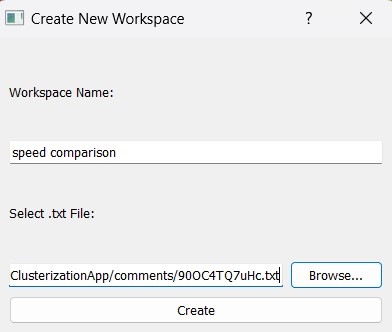
\includegraphics[width=0.5\textwidth]{./img/NewWorkspaceExampleFull.jpg}}
			\caption{Przykład wykonanego okna tworzenia nowego obszaru roboczego.}
			\label{fig:NewWorkspaceExampleFull}
		\end{figure}
	
	\section{Przykład ustawienia parametrów i metod}
	
		Ten przykład przedstawia różne kombinacje metod i ustawień dla konkretnego przypadku.
		
		\subsection{Przetwarzanie tekstu}
		
			Za pomocą przycisków \textbf{Previous} i \textbf{Next} można przeglądać zmiany ustawień przetwarzania tekstu oraz zobaczyć wyniki analizy częstotliwości i długości tekstu na wykresach.
			
		\subsubsection{Alpha}
			
		Rozważmy zastosowanie parametru \textbf{alpha}. Efekt użycia parametru \textbf{alpha} można wyraźnie zobaczyć na rysunkach \textbf{freq\_analysis} i \textbf{length\_analysis}. Na Rysunku \ref{fig:FreqTextParamsNone} wśród często występujących tokenów znajduje się duża liczba znaków specjalnych, podczas gdy na Rysunku \ref{fig:FreqTextParamsAlpha} pozostają tylko tokeny bez znaków specjalnych. Rysunki \ref{fig:LenTextParamsNone} i \ref{fig:LenTextParamsAlpha} pokazują, jak znacząco zmienia się średnia liczba tokenów w komentarzach. To pokazuje, że \textbf{alpha} działa poprawnie.
					
			
			\begin{figure}[ht]
				\centering
				\begin{minipage}{0.45\textwidth}
					\centering
					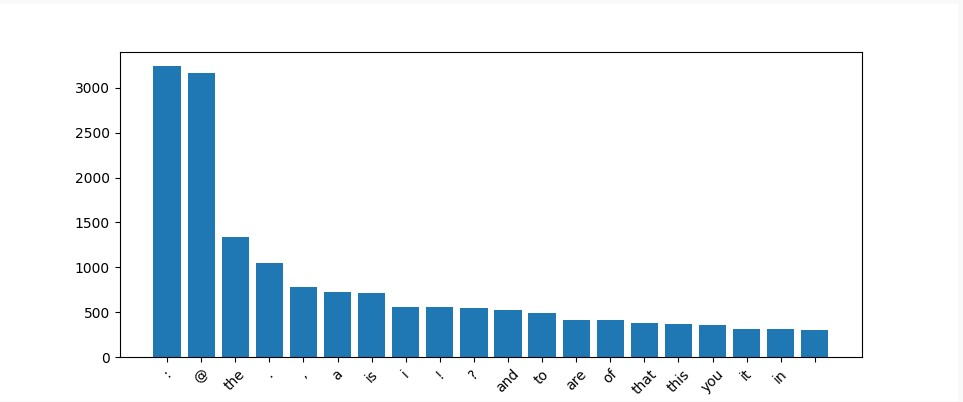
\includegraphics[width=\linewidth]{./img/FreqTextParamsNone.jpg}
					\caption{Przykład analizy częstotliwości tekstu bez TextProcessing.}
					\label{fig:FreqTextParamsNone}
				\end{minipage}\hfill
				\begin{minipage}{0.45\textwidth}
					\centering
					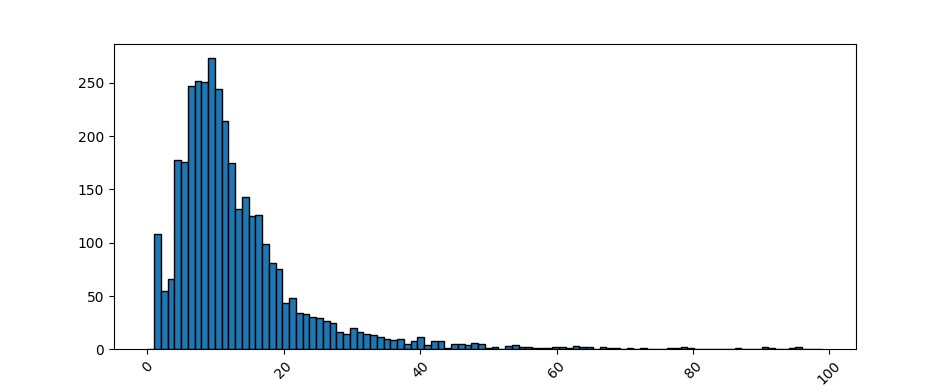
\includegraphics[width=\linewidth]{./img/LenTextParamsNone.jpg}
					\caption{Przykład analizy długości tekstu bez TextProcessing.}
					\label{fig:LenTextParamsNone}
				\end{minipage}
			\end{figure}
			
			
			\begin{figure}[ht]
				\centering
				\begin{minipage}{0.45\textwidth}
					\centering
					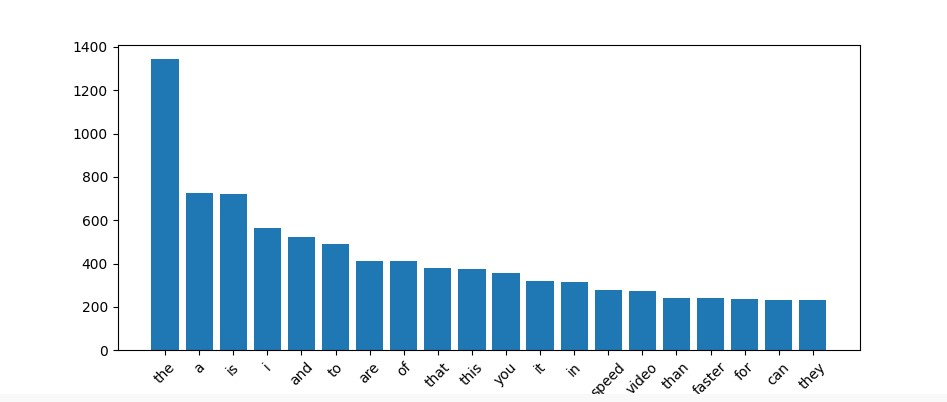
\includegraphics[width=\linewidth]{./img/FreqTextParamsAlpha.jpg}
					\caption{Przykład analizy częstotliwości tekstu z Alpha.}
					\label{fig:FreqTextParamsAlpha}
				\end{minipage}\hfill
				\begin{minipage}{0.45\textwidth}
					\centering
					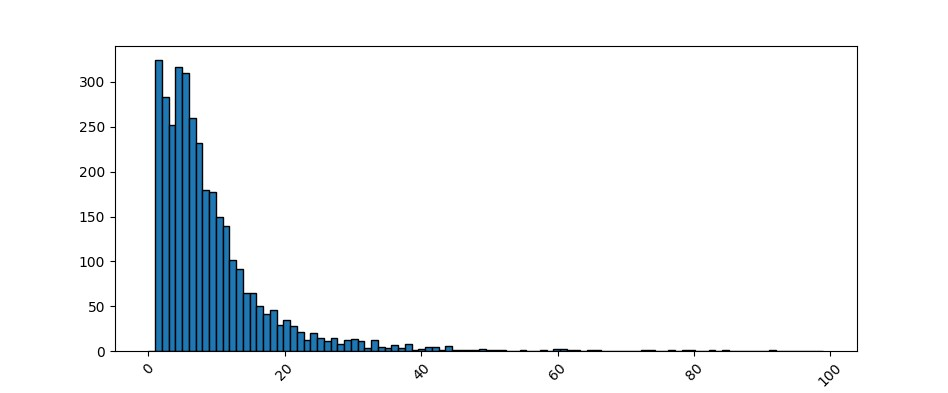
\includegraphics[width=\linewidth]{./img/LenTextParamsAlpha.jpg}
					\caption{Przykład analizy długości tekstu z Alpha.}
					\label{fig:LenTextParamsAlpha}
				\end{minipage}
			\end{figure}
			
			
		\subsubsection{Stop-words}
			
		Rozważmy zastosowanie parametru \textbf{stop-words}. Efekt użycia parametru \textbf{stop-words} można wyraźnie zobaczyć na wykresach \textbf{freq\_analysis} i \textbf{length\_analysis}. Rysunek \ref{fig:FreqTextParamsAlpha} zawiera dużą liczbę przyimków i artikeli wśród często występujących tokenów, podczas gdy na rysunku \ref{fig:FreqTextParamsAlphaStop} pozostają tylko rzeczowniki pospolite, które niosą ze sobą najwięcej informacji. Na rysunkach \ref{fig:LenTextParamsAlpha} i \ref{fig:LenTextParamsAlphaStop} pokazują, że średnia liczba tokenów w komentarzu również spada. Wskazuje to, że \textbf{stop-words} działają poprawnie.
			
			\begin{figure}[ht]
				\centering
				\begin{minipage}{0.45\textwidth}
					\centering
					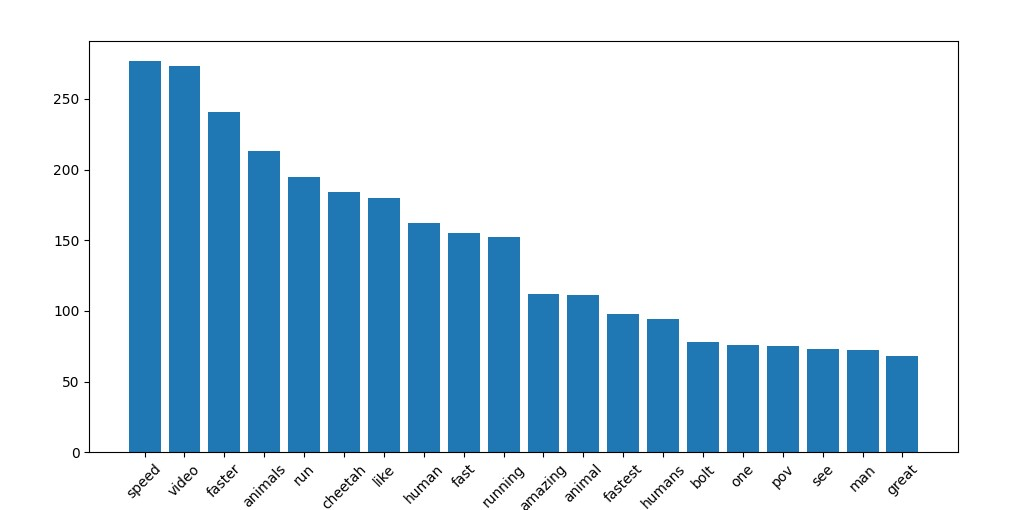
\includegraphics[width=\linewidth]{./img/FreqTextParamsAlphaStop.jpg}
					\caption{Przykład analizy częstotliwości tekstu z alpha i stop-words.}
					\label{fig:FreqTextParamsAlphaStop}
				\end{minipage}\hfill
				\begin{minipage}{0.45\textwidth}
					\centering
					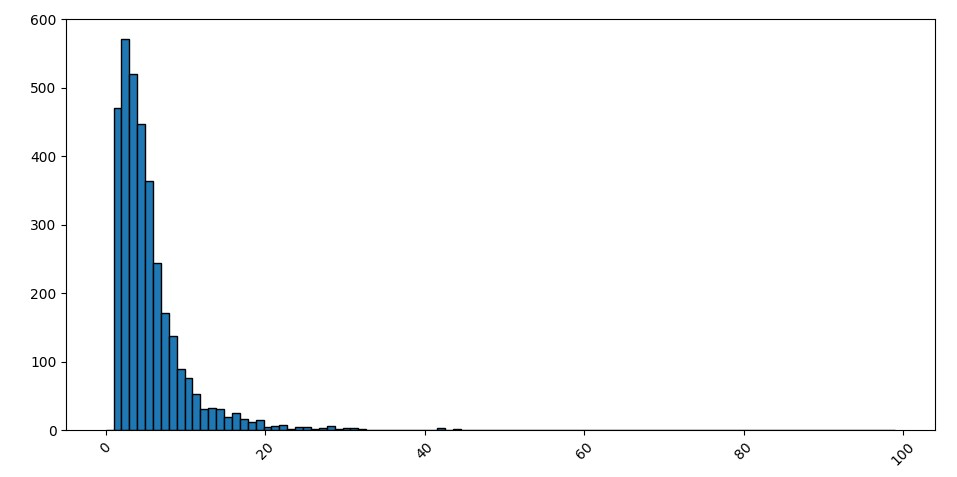
\includegraphics[width=\linewidth]{./img/LenTextParamsAlphaStop.jpg}
					\caption{Przykład analizy długości tekstu z alpha i stop-words.}
					\label{fig:LenTextParamsAlphaStop}
				\end{minipage}
			\end{figure}
		
		\subsubsection{Lemmatize}
		
		Rozważmy zastosowanie parametru \textbf{lemmatize}. Efekt jego użycia jest wyraźnie widoczny na wykresie \textbf{freq\_analysis}. Działanie parametru \textbf{lemmatize} najlepiej ilustruje łączenie form zwierząt \textbf{animals} i \textbf{animal}, co można zaobserwować na Rysunku \ref{fig:FreqTextParamsAlphaStop} oraz Rysunku \ref{fig:FreqTextParamsAlphaStopLem}. Po zastosowaniu lematyzacji, \textbf{animal} staje się najczęstszą formą. Podobne zmiany można zauważyć w przypadku \textbf{humans} i \textbf{human}.
			
			
			\begin{figure}[ht]
				\centering
				\begin{minipage}{0.45\textwidth}
					\centering
					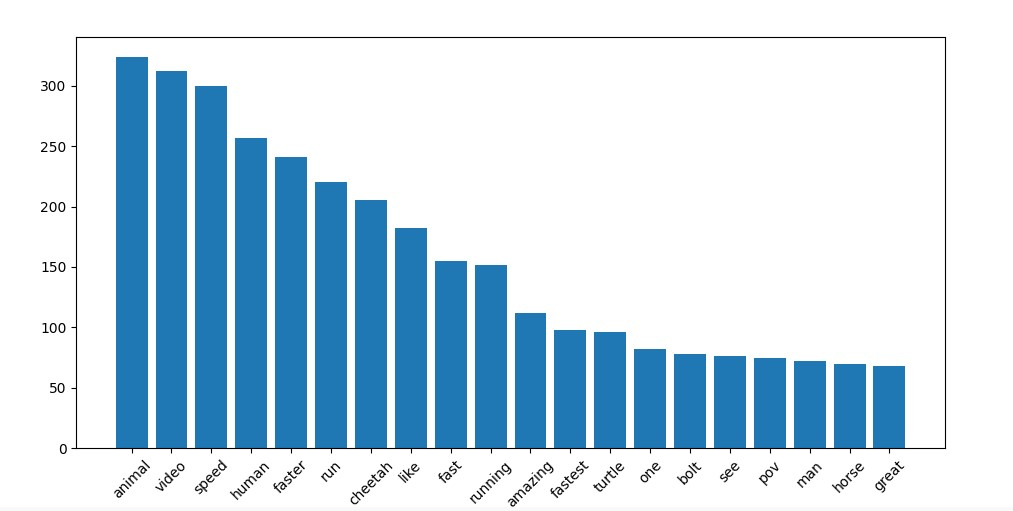
\includegraphics[width=\linewidth]{./img/FreqTextParamsAlphaStopLem.jpg}
					\caption{Przykład analizy częstotliwości tekstu z alpha i stop-words i lemmatize.}
					\label{fig:FreqTextParamsAlphaStopLem}
				\end{minipage}\hfill
				\begin{minipage}{0.45\textwidth}
					\centering
					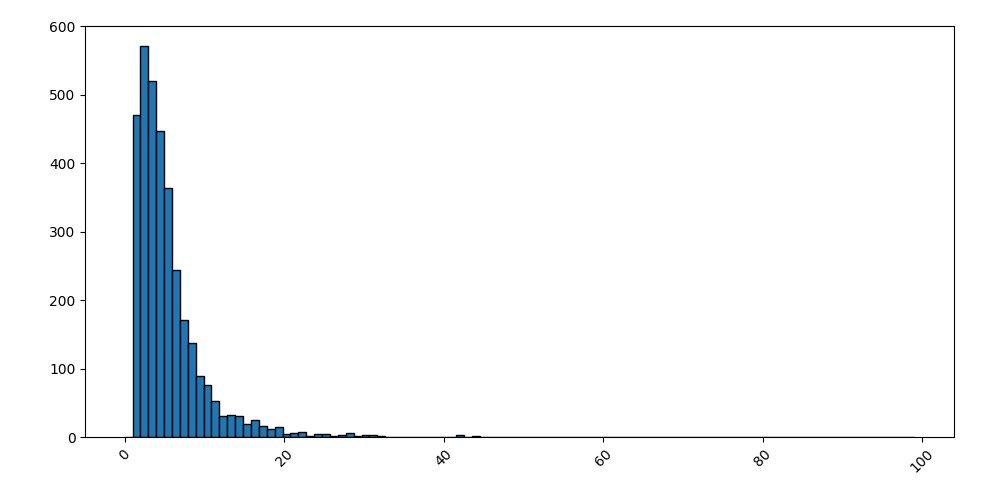
\includegraphics[width=\linewidth]{./img/LenTextParamsAlphaStopLem.jpg}
					\caption{Przykład analizy długości tekstu z alpha i stop-words i lemmatize.}
					\label{fig:LenTextParamsAlphaStopLem}
				\end{minipage}
			\end{figure}

		
		\subsection{Wektoryzacja}
			Wynik wektoryzacji możliwy do ocenienia dopiero po wizualizacji. W kolejnych sekcjach przedstawione wizualne wykorzystanie TF-IDF i Word2Vec z różnymi parametrami.
		
		\subsubsection{TF-IDF}
			Podczas korzystania z metody \textbf{TF-IDF} rozważmy dwa przypadki. Użycie domyślnych parametrów na Rysunku \ref{fig:tfstandard} i użycie parametrów (\textbf{max\_df} = 0.5, \textbf{min\_df} = 0.5) na Rysunku \ref{fig:tf0505}. W takich przypadkach analiza skupień jest praktycznie niemożliwa. Dane są bardzo mieszane, z najczęściej występującymi tokenami skupionymi w centrum i rzadko występującymi tokenami na krawędziach. Różnica przy zmianie parametrów nie jest bardzo widoczna, ale na Rysunku \ref{fig:tf0505} możemy zauważyć linie kierujące od środka do krawędzi, podczas gdy na Rysunku \ref{fig:tfstandard} 1 wykres jest równomiernie rozłożony na okręgu.
		
		\begin{figure}
			\centering
			\scalebox{1.0} {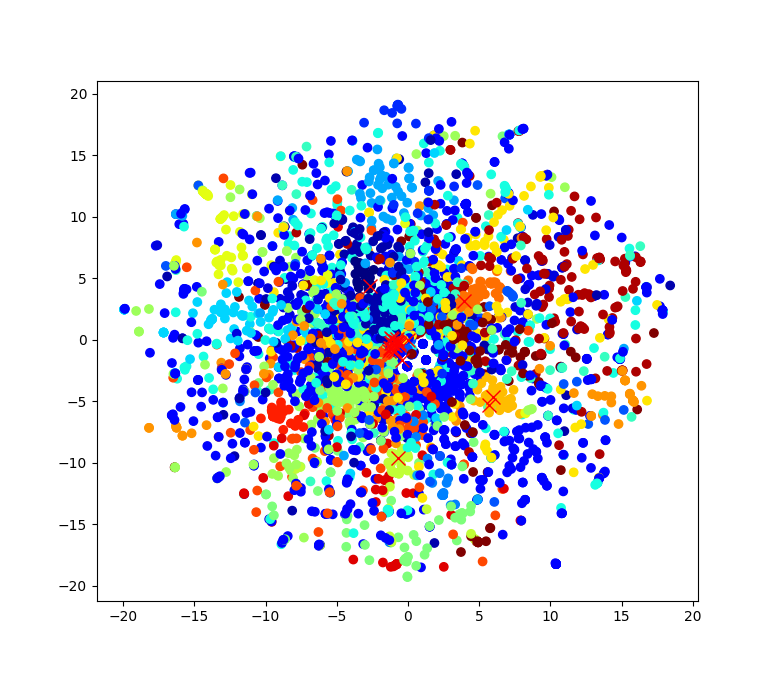
\includegraphics[width=0.5\textwidth]{./img/if-idfstandard.jpeg}}
			\caption{Przykład TF-IDF przy użyciu parametrów domyślnych.}
			\label{fig:tfstandard}
		\end{figure}
		
		\begin{figure}
			\centering
			\scalebox{1.0} {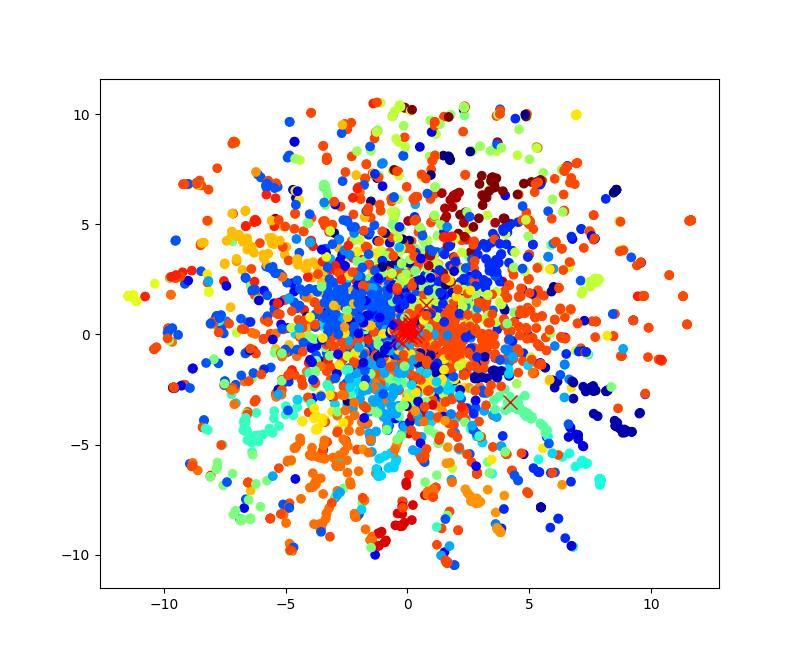
\includegraphics[width=0.5\textwidth]{./img/tf-idf0505.jpeg}}
			\caption{Przykład TF-IDF przy użyciu niestandardowych parametrów.}
			\label{fig:tf0505}
		\end{figure}
			
		
		\subsubsection{Word2Vec}
			Podczas korzystania z metody \textbf{Word2Vec} rozważmy dwa przypadki. Bardziej widoczne, gdy zmieniane są parametry \textbf{vector\_size}, gdzie wykres jest jakby rozciągnięty. Wykres z domyślnymi parametrami ilustrowany jest na Rysunku \ref{fig:w2v_standard} i jak wygląda na Rysunku \ref{fig:w2v_size500} z parametrami \textbf{vector\_size} = 500. Analiza wydajności klastrowania przy użyciu \textbf{Word2vec} staje się bardziej widoczna. Na Rysunku \ref{fig:w2v_size500} i Rysunku \ref{fig:w2v_standard} jest widoczny wyraźny podział na różne klastry.
		 
		
		\begin{figure}[ht]
			\centering
			\begin{minipage}{0.45\textwidth}
				\centering
				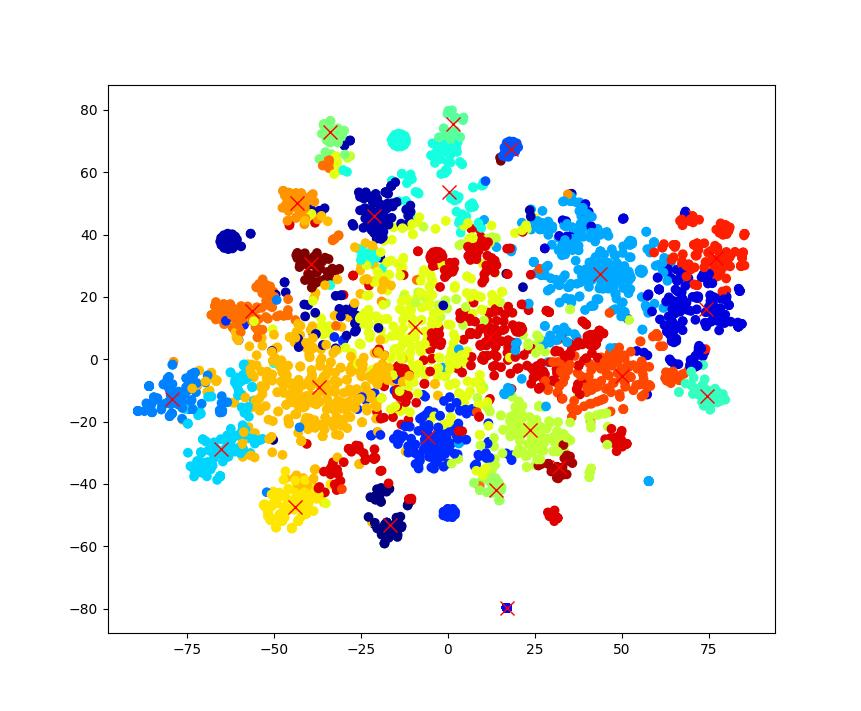
\includegraphics[width=\linewidth]{./img/w2v_standard.jpeg}
				\caption{Przykład Word2Vec przy vector\_size = 150.}
				\label{fig:w2v_standard}
			\end{minipage}\hfill
			\begin{minipage}{0.45\textwidth}
				\centering
				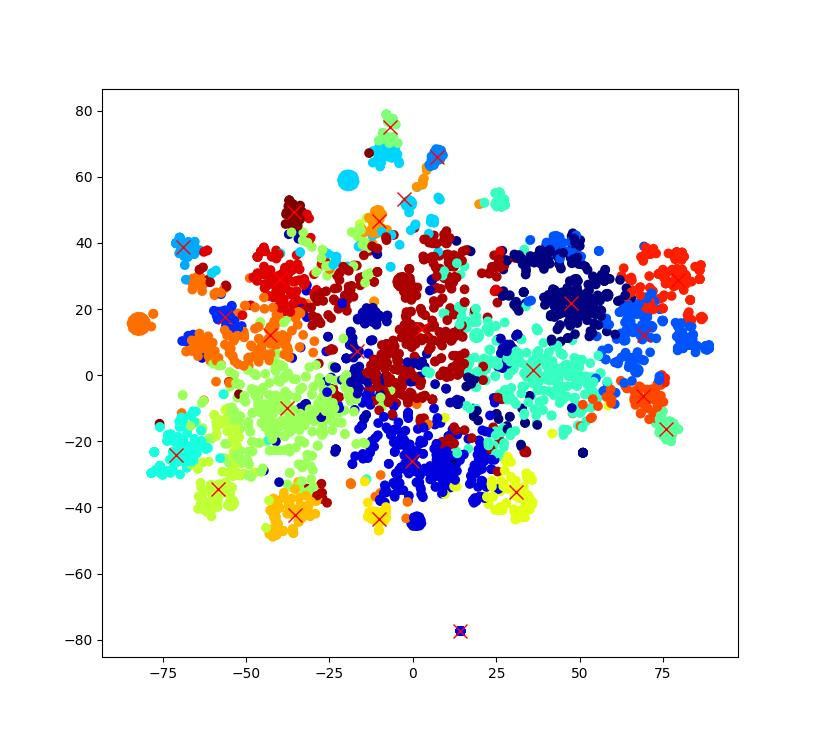
\includegraphics[width=\linewidth]{./img/w2v_size500.jpeg}
				\caption{Przykład Word2Vec przy vector\_size = 500.}
				\label{fig:w2v_size500}
			\end{minipage}
		\end{figure}
		
		\subsection{Klasteryzacja}
		
		\subsubsection{K-means}
		
		Rozważmy trzy przypadki zastosowania algorytmu \textbf{K-means} z liczbą klastrów wynoszącą odpowiednio 5, 15 i 35, przedstawione na Rysunkach \ref{fig:w2vkmeans5}, \ref{fig:w2vkmeans15} i \ref{fig:w2vkmeans35}.
		
		W pierwszym przypadku  wyraźnie widać, że liczba klastrów jest niewystarczająca. Poszczególne grupy nie są prawidłowo odwzorowane, co prowadzi do wewnętrznego podziału w obrębie pojedynczych klastrów.
		
		W drugim przypadku również liczba klastrów jest zbyt mała. Pomimo zwiększenia liczby klastrów, nadal występują problemy z ich podziałem, co sugeruje, że ilość klastrów jest niewystarczająca do pełnego odwzorowania struktury danych.
		
		W trzecim przypadku liczba klastrów wynosi 35 i jest już zbliżona do optymalnej. Niemniej jednak, zauważamy, że w niektórych miejscach kluczowe regiony są dzielone na mniejsze, zbyteczne klastry, co wskazuje na nieznaczne przekroczenie wymaganej liczby klastrów.
		
		
		\begin{figure}
			\centering
			\scalebox{1.0} {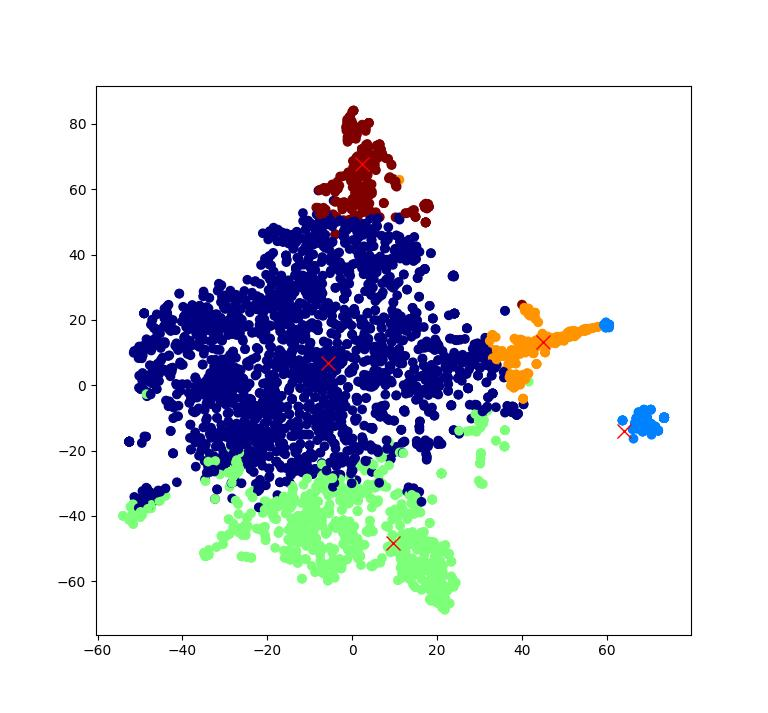
\includegraphics[width=0.5\textwidth]{./img/w2vkmeans5.jpeg}}
			\caption{Przykład K-means przy n\_clusters = 5.}
			\label{fig:w2vkmeans5}
		\end{figure}
		
		\begin{figure}
			\centering
			\scalebox{1.0} {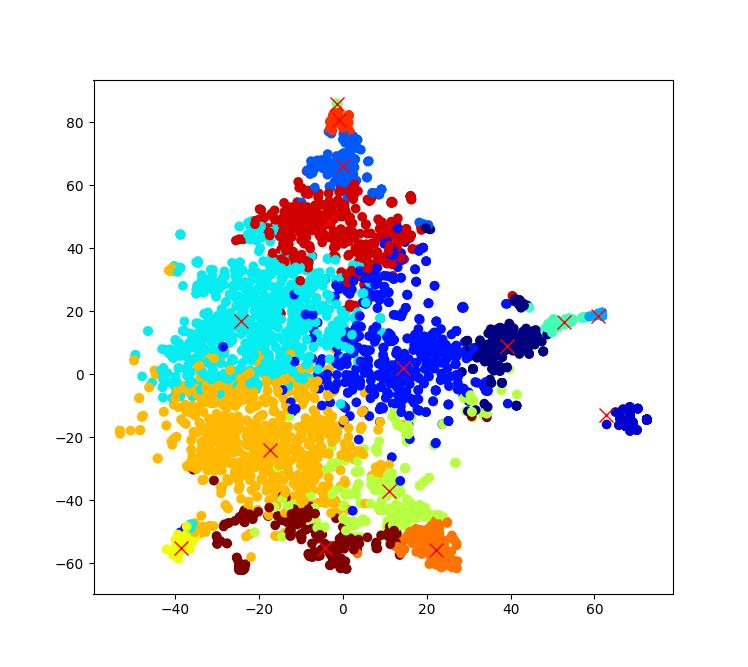
\includegraphics[width=0.5\textwidth]{./img/w2vkmeans15.jpeg}}
			\caption{Przykład K-means przy n\_clusters = 15.}
			\label{fig:w2vkmeans15}
		\end{figure}
		
		\begin{figure}
			\centering
			\scalebox{1.0} {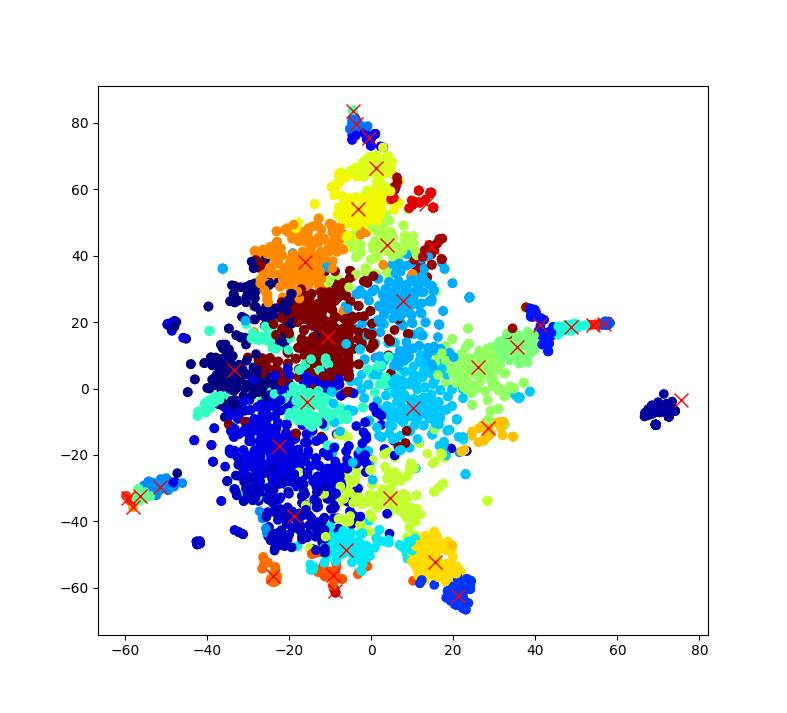
\includegraphics[width=0.5\textwidth]{./img/w2vkmeans35.jpeg}}
			\caption{Przykład K-means przy n\_clusters = 35.}
			\label{fig:w2vkmeans35}
		\end{figure}
		
		
		\subsubsection{DBSCAN}
		
		Rozważmy cztery przypadki pracy z DBSCAN. Rozważmy zmianę \textbf{eps} jak na rysunkach \ref{fig:w2cdbscan4_0-05} i \ref{fig:w2cdbscan4_0-075}. I zmianę \textbf{min\_pts} na rysunkach \ref{fig:w2cdbscan2_0-05} i \ref{fig:w2cdbscan10_0-05}. We wszystkich przypadkach widzimy, że DBSCAN jest bardzo wrażliwy na wybór parametrów. Na Rysunku \ref{fig:w2cdbscan4_0-05} i Rysunku \ref{fig:w2cdbscan10_0-05}  większość komentarzy nie jest zawarta w żadnym klastrze, a większość klastrów składa się z bardzo małej liczby komentarzy. Na Rysunku \ref{fig:w2cdbscan4_0-075} i Rysunku \ref{fig:w2cdbscan2_0-05}, ponieważ parametry były bardzo korzystne dla grupowania, większość komentarzy została skupiona w jednym dużym klastrze.
		
			\begin{figure}[ht]
			\centering
			\begin{minipage}{0.45\textwidth}
				\centering
				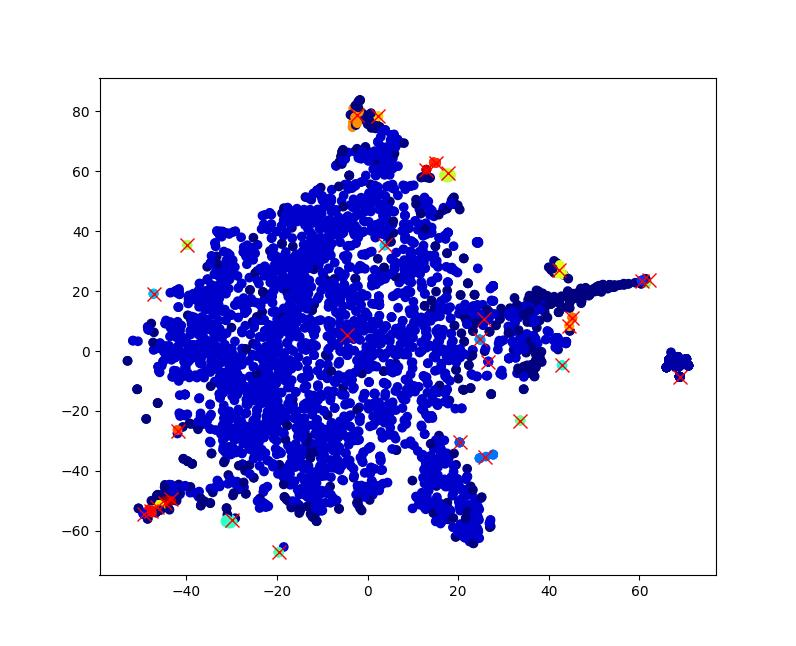
\includegraphics[width=\linewidth]{./img/w2cdbscan4_0-05.jpeg}
				\caption{Przykład DBSCAN przy eps = 4 i min\_pts = 0.05.}
				\label{fig:w2cdbscan4_0-05}
			\end{minipage}\hfill
			\begin{minipage}{0.45\textwidth}
				\centering
				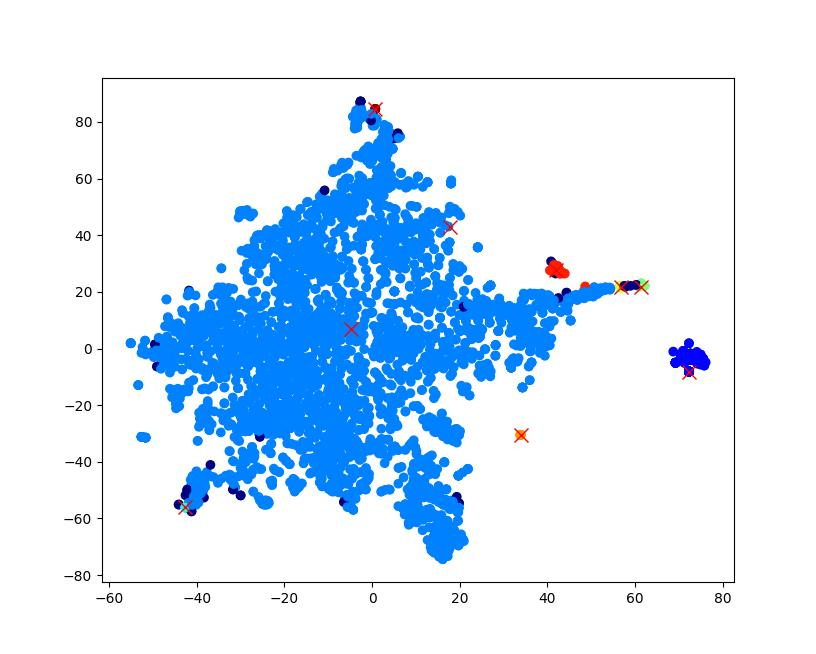
\includegraphics[width=\linewidth]{./img/w2cdbscan4_0-075.jpeg}
				\caption{Przykład DBSCAN przy eps = 4 i min\_pts = 0.075.}
				\label{fig:w2cdbscan4_0-075}
			\end{minipage}
		\end{figure}
		
			\begin{figure}[ht]
			\centering
			\begin{minipage}{0.45\textwidth}
				\centering
				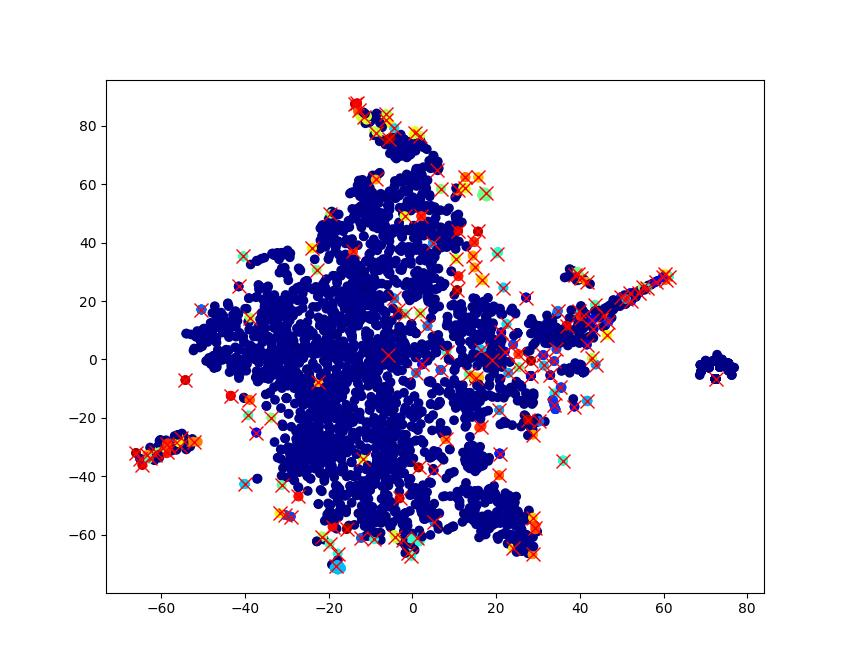
\includegraphics[width=\linewidth]{./img/w2cdbscan2_0-05.jpeg}
				\caption{Przykład DBSCAN przy eps = 2 i min\_pts = 0.05.}
				\label{fig:w2cdbscan2_0-05}
			\end{minipage}\hfill
			\begin{minipage}{0.45\textwidth}
				\centering
				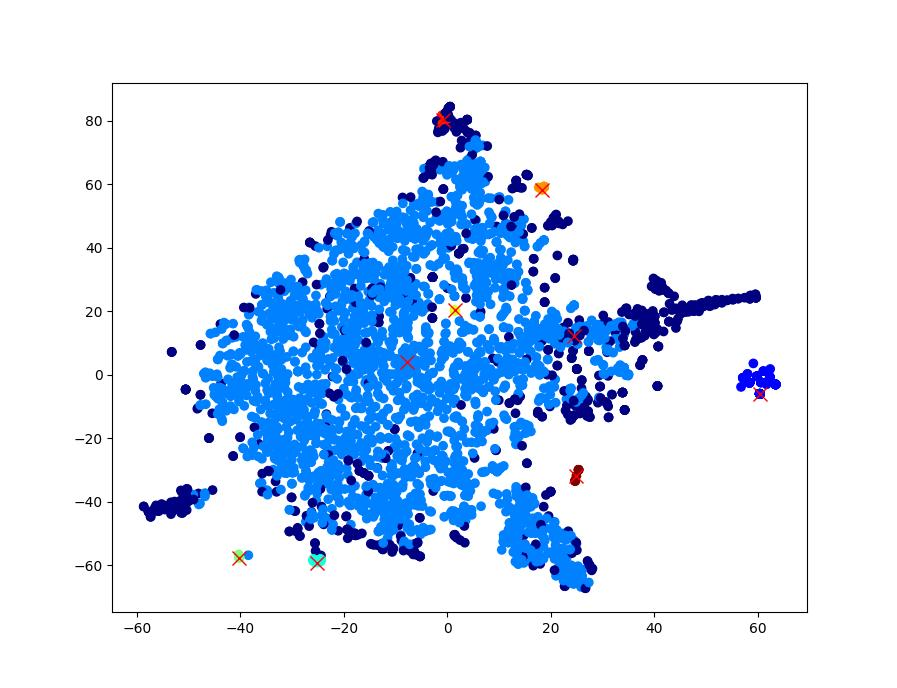
\includegraphics[width=\linewidth]{./img/w2cdbscan10_0-05.jpeg}
				\caption{Przykład DBSCAN przy eps = 10 i min\_pts = 0.05.}
				\label{fig:w2cdbscan10_0-05}
			\end{minipage}
		\end{figure}
	
	
	\subsection{Analiza wynkiow pracy}
		Przyjrzyjmy się analizie danych dla tego przykładu przy użyciu parametrów \textbf{Word2vec}, grupowania z parametrami \textbf{K-means} i wszystkich metod przetwarzania tekstu.
		
		Wynik grupowania pokazano na Rysunku \ref{fig:resultAll}. 
		Rysunek \ref{fig:resultbolt} przedstawia grupę komentarzy oddzielonych od części ogólnej, w oparciu o informacje o centrum klastra \textbf{bolt} i komentarze z tego obszaru, wydaje się, że komentarze te często wspominają o \textbf{Usain Bolt}.  
		Również  bardziej podobne komentarze znajdują się bliżej siebie, jak na Rysunku \ref{fig:resultamazing} \textbf{Amaizing} i rysunku \ref{fig:resultHuman} \textbf{human}. 
		Grupa \textbf{Amazing} na Rysunku \ref{fig:resultamazing} i grupa \textbf{Content} na Rysunku \ref{fig:resultContent}, gdzie często wspomina się o \textbf{Video Amazing}, znajdują się blisko siebie.
		
			\begin{figure}[ht]
			\centering
			\begin{minipage}{0.45\textwidth}
				\centering
				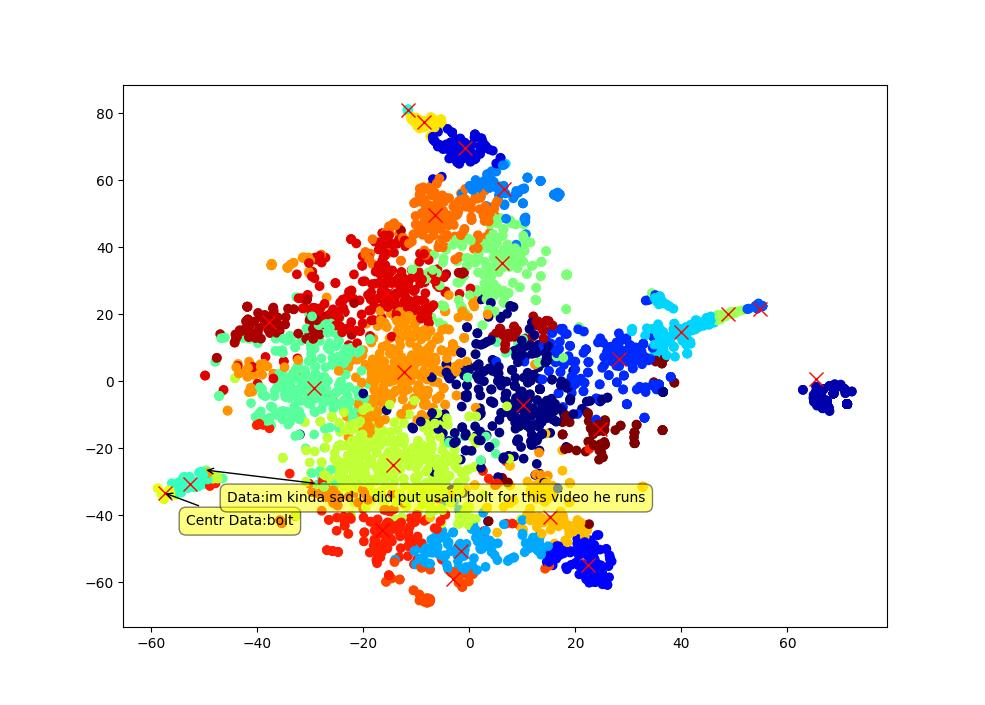
\includegraphics[width=\linewidth]{./img/resultbolt.jpeg}
				\caption{Przykład wyniku pracy.}
				\label{fig:resultbolt}
			\end{minipage}\hfill
			\begin{minipage}{0.45\textwidth}
				\centering
				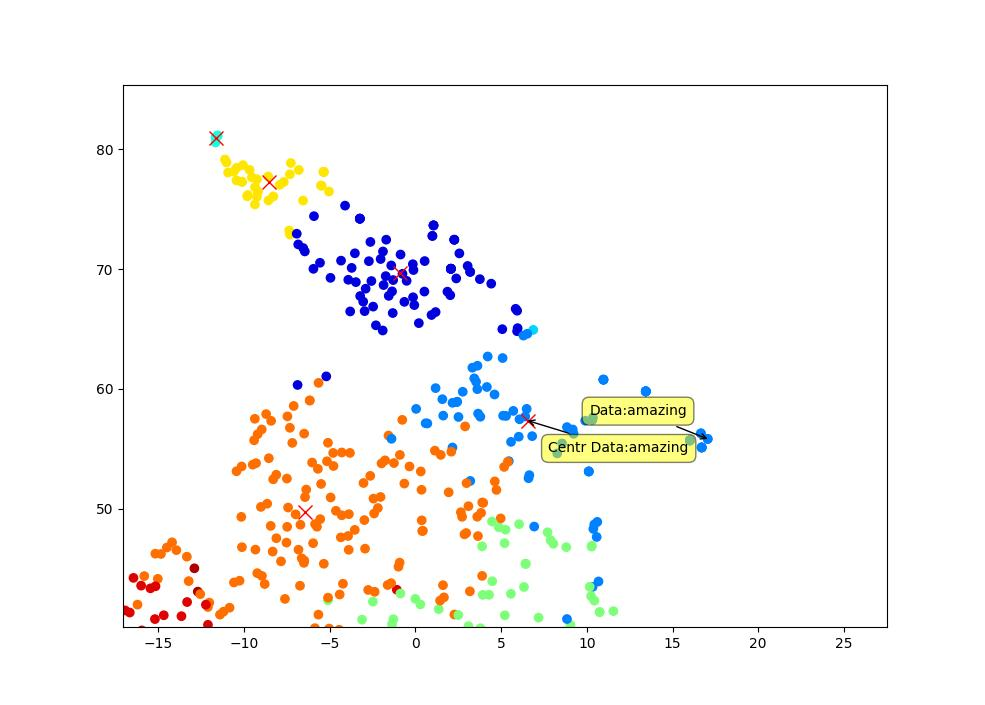
\includegraphics[width=\linewidth]{./img/resultAmazing.jpeg}
				\caption{Przykład wyniku pracy.}
				\label{fig:resultamazing}
			\end{minipage}
		\end{figure}
		
			\begin{figure}[ht]
			\centering
			\begin{minipage}{0.45\textwidth}
				\centering
				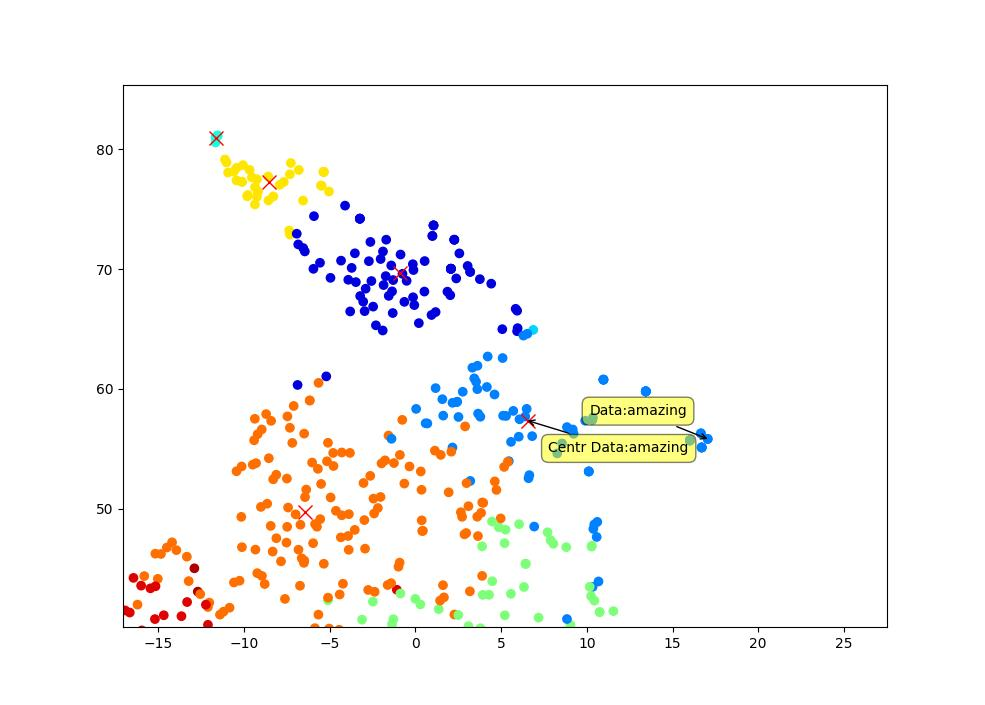
\includegraphics[width=\linewidth]{./img/resultAmazing.jpeg}
				\caption{Przykład wyniku pracy.}
				\label{fig:resultAll}
			\end{minipage}\hfill
			\begin{minipage}{0.45\textwidth}
				\centering
				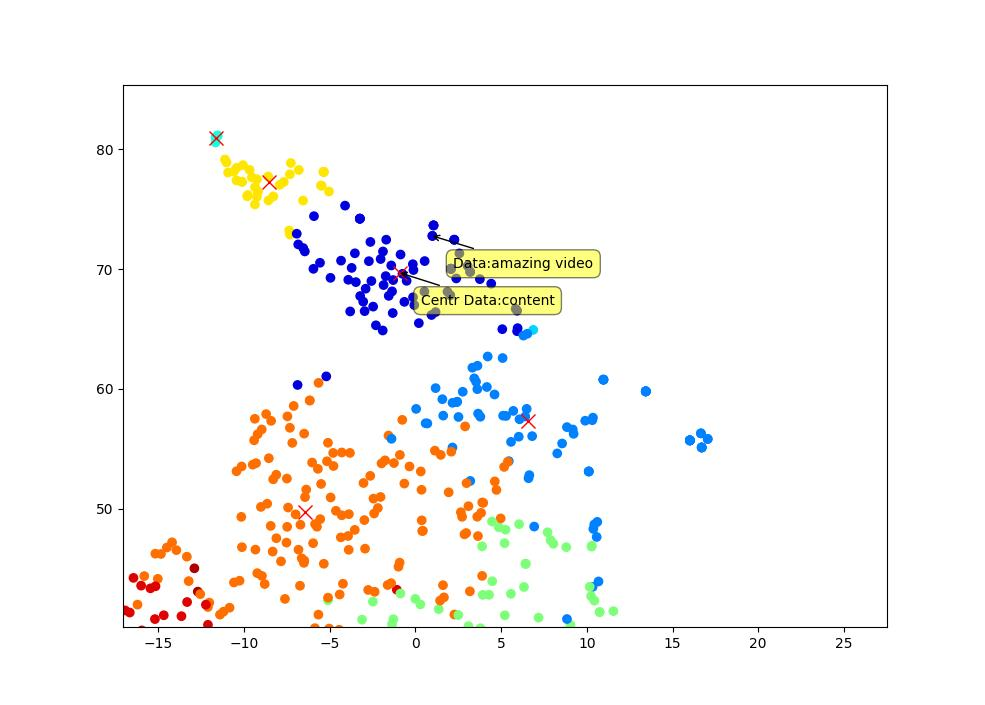
\includegraphics[width=\linewidth]{./img/resultContent.jpeg}
				\caption{Przykład wyniku pracy.}
				\label{fig:resultContent}
			\end{minipage}
		\end{figure}
		
			\begin{figure}[ht]
			\centering
			\begin{minipage}{0.45\textwidth}
				\centering
				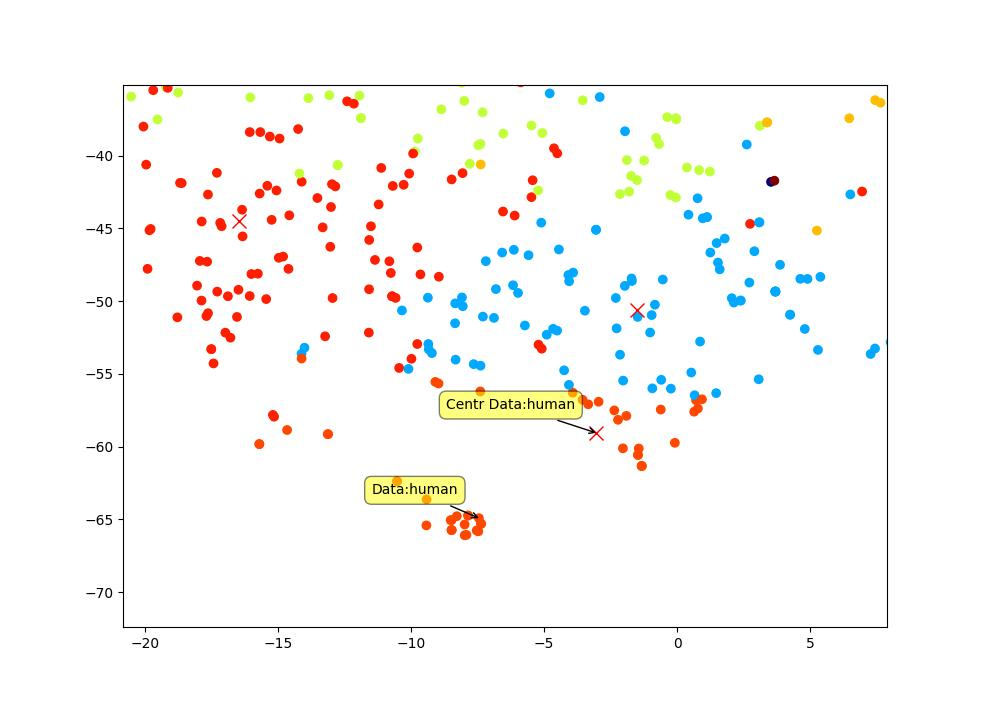
\includegraphics[width=\linewidth]{./img/resultHuman.jpeg}
				\caption{Przykład wyniku pracy.}
				\label{fig:resultHuman}
			\end{minipage}\hfill
			\begin{minipage}{0.45\textwidth}
				\centering
				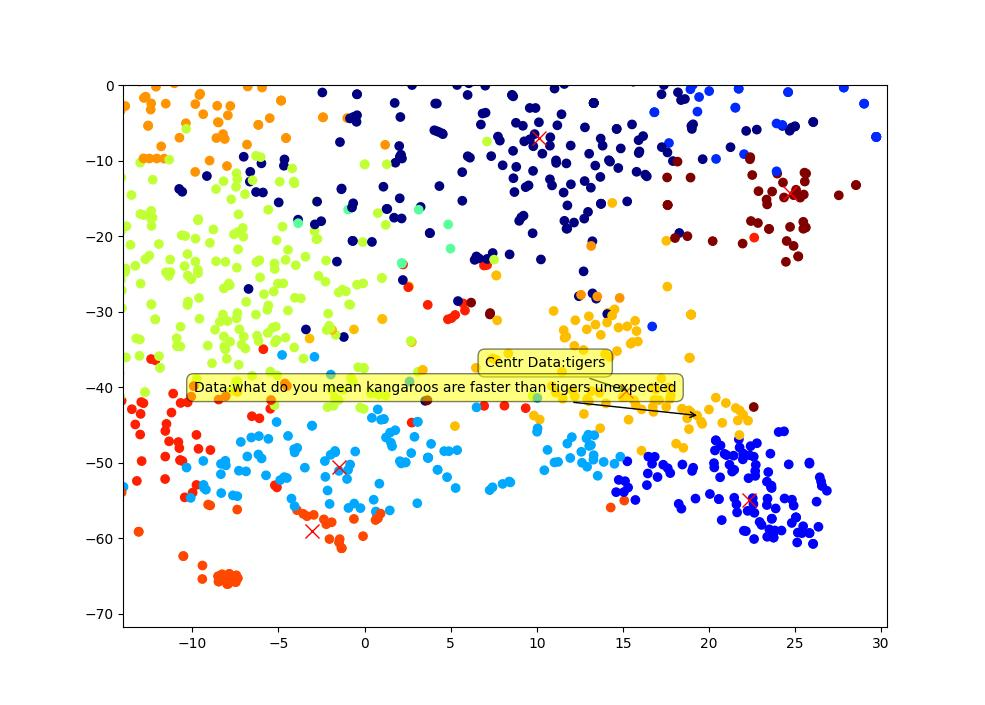
\includegraphics[width=\linewidth]{./img/resultTigers.jpeg}
				\caption{Przykład wyniku pracy.}
				\label{fig:resultTigers}
			\end{minipage}
		\end{figure}
		
